\documentclass[11pt,a4paper]{article}

\usepackage[utf8]{inputenc}
\usepackage[T1]{fontenc}
\usepackage[spanish,es-tabla]{babel}
\usepackage{lmodern}
\usepackage[margin=2.5cm]{geometry}
\usepackage{amsmath,amssymb}
\usepackage{graphicx}
\usepackage{booktabs}
\usepackage{array}
\usepackage{multirow}
\usepackage{caption}
\usepackage{float}
\usepackage{microtype}
\usepackage{xcolor}
\usepackage[colorlinks=true,linkcolor=blue!50!black,citecolor=blue!50!black,urlcolor=blue!50!black]{hyperref}

\captionsetup{font=small,labelfont=bf}
\setlength{\parskip}{0.4em}

\title{\textbf{Predicción de demanda de pasajeros en transporte urbano a 30, 60 y 120 minutos con datos de sensores y gradient boosting}\\[0.4em]
\large Caso de tres rutas de SOBUSA (2023--2025)}

\author{Daza Roger: \texttt{polora@uninorte.edu.co}\\
Del Sole Matteo: \texttt{msole@uninorte.edu.co}\\
Romero Rafael: \texttt{arafaelr@uninorte.edu.co}\\[0.3em]
\small Universidad del Norte, Barranquilla}

\date{\today}

\begin{document}
\maketitle

\begin{abstract}
Anticipar cuántos pasajeros subirán a un bus en las próximas horas permite ajustar la oferta de viajes antes de que se produzca el desajuste. En este trabajo se construye un sistema de predicción de las subidas de pasajeros por ruta en franjas de 15 minutos, con horizontes de 30, 60 y 120 minutos, para tres rutas del operador SOBUSA. Se usan 176 millones de lecturas de sensores de conteo (2023--2025), a las que se aplican reglas de calidad derivadas de un análisis exploratorio: días sin lecturas, saltos del contador y un sensor de bajadas poco fiable. Se entrena un modelo XGBoost con objetivo de Poisson por horizonte, con 22 variables que usan únicamente información disponible en el instante de predecir, lo cual se verifica con una prueba de alteración del futuro. En un periodo de prueba posterior al de entrenamiento (junio a diciembre de 2025), el modelo reduce el WAPE de 15,8\,\% (promedio de las cuatro semanas previas) a 10,3\,\%, 10,7\,\% y 11,1\,\% para los horizontes de 30, 60 y 120 minutos. La mejora proviene sobre todo del uso de tres años de datos limpios de sensores y, en menor medida, de las variables de estacionalidad anual, nivel reciente y oferta. En días especiales (festivos, Semana Santa) el error sigue siendo mayor (15--18\,\%), aunque la línea base supera el 100\,\% en esos días. Para el despliegue, cada modelo se reentrena con los tres años de datos y se sirve mediante un servicio web que reutiliza el mismo código de variables del entrenamiento.
\end{abstract}

\noindent\textbf{Palabras clave:} predicción de demanda, transporte público, series de tiempo, XGBoost, SHAP, conteo de pasajeros.

%-----------------------------------------------------------------------
\section{Introducción}
%-----------------------------------------------------------------------

La demanda de pasajeros en el transporte público urbano sigue patrones regulares (picos de la mañana y de la tarde, diferencias entre días hábiles y fines de semana), pero también sufre alteraciones que el calendario no siempre anuncia: festivos, Carnaval, partidos de la selección nacional, lluvias o paros. Un operador que conoce con antelación la demanda esperada puede reforzar o reducir viajes, y evaluar si la programación del día se ajusta a lo que ocurre en la calle.

Este trabajo aborda el problema de predecir, para cada ruta, el número de pasajeros que suben en una franja de 15 minutos con una antelación de 30, 60 y 120 minutos. Los datos provienen del reto de datos de SOBUSA e incluyen las lecturas de los sensores de pasajeros de los buses entre enero de 2023 y diciembre de 2025.

Las contribuciones son las siguientes:
\begin{enumerate}
  \item Un diagnóstico de calidad de los datos de sensores que identifica tres problemas concretos (días sin lecturas, saltos del contador y bajadas inconsistentes) y las reglas para tratarlos.
  \item Un conjunto de 22 variables sin fuga de información, con una prueba directa que comprueba que ninguna usa datos posteriores a la referencia de predicción.
  \item Un modelo por horizonte que mejora entre 30\,\% y 35\,\% el error de la mejor línea base, con una ablación que cuantifica el aporte de cada grupo de variables.
  \item Un servicio web que sirve los modelos y recalcula las variables con el mismo código usado para entrenar.
\end{enumerate}

%-----------------------------------------------------------------------
\section{Datos}
%-----------------------------------------------------------------------

\subsection{Fuentes}

Se revisaron las 30 tablas de la base de datos del operador. La fuente principal es la tabla \texttt{conteo\_pasajeros\_destino}, que guarda la lectura del sensor de pasajeros de cada bus aproximadamente cada minuto (176 millones de filas entre enero de 2023 y diciembre de 2025). Las lecturas se agregan por ruta y por franja de 15 minutos según la hora real de cada subida, no según la hora de salida del bus. Esto es importante porque un viaje dura en promedio unas tres horas (mediana de 198 minutos), de modo que asignar sus pasajeros a la hora de salida desplazaría la demanda.

Como fuentes complementarias se usan la programación de viajes (\texttt{progvehiculos}, 565 mil viajes) y las tablas de calendario con festivos, temporadas (Precarnaval, Carnaval, Semana Santa) y eventos con su porcentaje de impacto declarado. Tras la agregación quedan 243\,508 franjas de 15 minutos con servicio y 43,8 millones de subidas para tres rutas: la Ruta 2 (Silencio), la Ruta 16 (Carrera 54) y la Ruta 21 (Calle 72).

La tabla \texttt{timbradas\_segmentos}, que daba subidas por segmento de 500 m, se descartó por dos razones. Solo cubre ocho semanas (1 de enero a 27 de febrero de 2023) y sus horas están desplazadas respecto de los sensores y los despachos: la correlación franja a franja entre ambas fuentes sube de 0,47 a 0,71 al correr los sensores dos horas. En una comparación de totales diarios, las dos fuentes difieren en menos de 1\,\% para la Ruta 16, y la suma de lecturas del sensor por viaje tiene correlación de 0,9999 con el número de pasajeros registrado en la programación, lo que respalda la fiabilidad de los sensores como fuente.

\subsection{Calidad de los datos}

El análisis exploratorio encontró tres problemas que se tratan antes de modelar.

\paragraph{Días sin lecturas.} El último día de cada mes la tabla de sensores está casi vacía (mediana de 15 lecturas frente a unas 180\,000 en un día normal), aunque los viajes sí se realizaron. Se trata de un hueco de la extracción y no de ausencia de demanda. Un día con menos del 5\,\% de las lecturas habituales de su ruta se marca como \emph{faltante} y no como cero; de lo contrario el modelo aprendería que la demanda desaparece a fin de mes. Afecta a 107 días-ruta.

\paragraph{Lecturas imposibles.} Una lectura de cerca de un minuto registra casi siempre entre 1 y 4 subidas, pero hay 38 franjas (0,016\,\%) con lecturas de miles de subidas, producidas por saltos del contador acumulado (el máximo observado supera las 97\,000 subidas en una lectura). Se descarta toda franja en la que alguna lectura supera 90 subidas, que es más de lo que cabe en un bus.

\paragraph{Bajadas no fiables.} En un recorrido completo bajan tantas personas como suben. Sin embargo, la Ruta 21 registra 2,3 veces más bajadas que subidas en 2023 y 1,8 veces en 2024, y la Ruta 16 un 16\,\% más en 2025. Por ello las bajadas no se usan ni como objetivo ni como variable.

Entre 7\,\% y 9\,\% de los viajes programados se cancelan cada año, pero esto no afecta al objetivo, pues los sensores solo registran viajes realizados.

\subsection{Patrones de la demanda}

\paragraph{Tendencia.} La demanda cae entre 3\,\% y 9\,\% por año en las tres rutas (Figura~\ref{fig:tendencia}); a la vez disminuyen los viajes por día y los pasajeros por viaje. Un modelo basado en árboles no extrapola tendencias, por lo que necesita una variable de nivel reciente para no quedar anclado al nivel de 2023.

\begin{figure}[H]
  \centering
  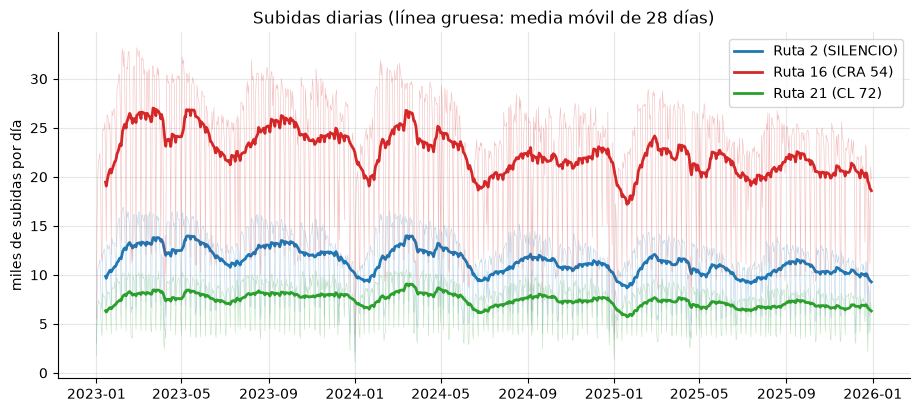
\includegraphics[width=0.85\textwidth]{fig/tendencia.png}
  \caption{Subidas diarias por ruta, 2023--2025. La línea gruesa es la media móvil de 28 días.}
  \label{fig:tendencia}
\end{figure}

\paragraph{Estacionalidad anual.} Una vez quitada la tendencia, enero, junio--julio y diciembre quedan por debajo del promedio (vacaciones escolares y universitarias), y febrero--mayo y agosto--septiembre por encima. La forma se repite los tres años, lo que justifica incluir el día del año y la demanda de la misma franja 52 semanas antes.

\paragraph{Patrón semanal y calendario.} El sábado equivale a 81\,\% de un día hábil, el domingo a 46\,\% y un festivo a 41\,\%. Los días centrales de Carnaval (lunes y martes) dejan la demanda en 35--42\,\% de lo normal y se comportan como festivo; la Semana Santa la deja en 51--60\,\%. El Precarnaval, en cambio, la \emph{aumenta} entre 5\,\% y 24\,\%. Las fiestas patronales no mueven la demanda de estas rutas. En su ventana horaria, los partidos de la selección reducen la demanda entre 17\,\% y 37\,\%, y la Guacherna entre 6\,\% y 19\,\%.

\paragraph{Perfil dentro del día.} Los días hábiles tienen dos picos (6--7 h y 17 h); el fin de semana el pico de la mañana se aplana y se desplaza (Figura~\ref{fig:perfil}). La forma cambia con la ruta y el tipo de día.

\begin{figure}[H]
  \centering
  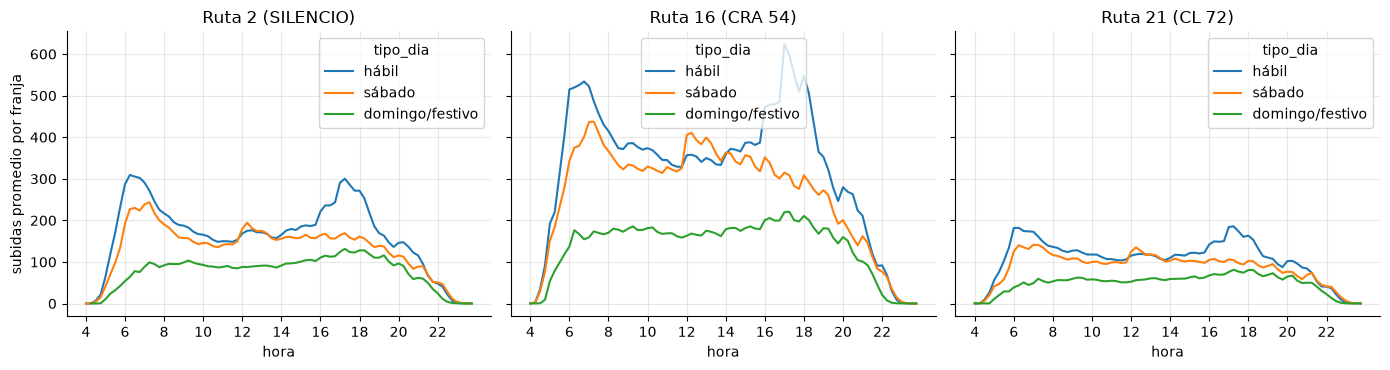
\includegraphics[width=\textwidth]{fig/perfil.png}
  \caption{Subidas promedio por franja de 15 minutos según la hora y el tipo de día, para cada ruta.}
  \label{fig:perfil}
\end{figure}

\paragraph{Qué información predice mejor.} La Tabla~\ref{tab:corr} muestra la correlación de las subidas de una franja con el dato de distintos rezagos. A 30 minutos el dato más reciente (0,82--0,89) vale tanto como el promedio de cuatro semanas (0,83--0,88); a dos horas el dato reciente casi pierde su valor (0,31--0,43) y domina el patrón habitual. El dato de un año antes (0,77--0,85) es tan informativo como el de una semana antes, lo que confirma que la estacionalidad anual es real.

\begin{table}[H]
  \centering
  \caption{Correlación entre las subidas de una franja y el dato con distinto rezago, por ruta.}
  \label{tab:corr}
  \small
  \begin{tabular}{lrrrrrrrr}
    \toprule
    Ruta & 15 min & 30 min & 1 h & 2 h & 1 día & 7 días & 364 días & Prom. 4 sem. \\
    \midrule
    2  & 0,932 & 0,867 & 0,671 & 0,311 & 0,720 & 0,833 & 0,841 & 0,880 \\
    16 & 0,947 & 0,893 & 0,749 & 0,432 & 0,691 & 0,836 & 0,846 & 0,882 \\
    21 & 0,881 & 0,815 & 0,651 & 0,369 & 0,632 & 0,760 & 0,767 & 0,832 \\
    \bottomrule
  \end{tabular}
\end{table}

%-----------------------------------------------------------------------
\section{Metodología}
%-----------------------------------------------------------------------

\subsection{Definición del problema}

Sea $y_{r,t}$ el número de subidas en la ruta $r$ durante la franja de 15 minutos que empieza en $t$. Para un horizonte $h \in \{30, 60, 120\}$ minutos, se busca estimar $y_{r,t}$ usando solo información disponible en el instante de referencia $t-h$. Se entrena un modelo independiente por horizonte, $\hat{y}_{r,t} = f_h(\mathbf{x}_{r,t})$, porque la utilidad de cada variable cambia con la antelación.

\subsection{Variables}

Las 22 variables se agrupan en cuatro familias (Tabla~\ref{tab:vars}). Las del calendario pueden mirar la franja $t$ porque se conocen con anticipación. Las que dependen de lo observado usan datos hasta $t-h$ como máximo.

\begin{table}[H]
  \centering
  \caption{Variables del modelo. $h$ es el horizonte expresado en franjas de 15 minutos.}
  \label{tab:vars}
  \small
  \renewcommand{\arraystretch}{1.15}
  \begin{tabular}{p{2.3cm} p{3.6cm} p{8.2cm}}
    \toprule
    Grupo & Variable & Definición \\
    \midrule
    Calendario & \texttt{id\_ruta} & Ruta (2, 16 o 21). \\
     & \texttt{minuto\_dia} & Minuto del día de la franja $t$. \\
     & \texttt{dia\_semana}, \texttt{tipo\_dia} & Día de la semana; hábil, sábado o domingo/festivo (lunes y martes de Carnaval cuentan como festivo). \\
     & \texttt{mes}, \texttt{dia\_del\_anio} & Posición en el año. \\
     & \texttt{es\_festivo}, \texttt{precarnaval}, \texttt{carnaval\_central}, \texttt{semana\_santa} & Indicadores de temporada. \\
     & \texttt{impacto\_evento} & Porcentaje de impacto declarado del evento activo en la franja. \\
    \addlinespace
    Reciente & \texttt{lag\_h}, \texttt{lag\_h\_mas\_1} & Subidas en $t-h$ y $t-h-1$. \\
     & \texttt{media\_1h\_previa} & Media de las cuatro franjas hasta $t-h$. \\
     & \texttt{ratio\_hoy} & Subidas acumuladas del día hasta $t-h$ sobre lo habitual a esa hora (promedio de cuatro semanas). \\
     & \texttt{nivel\_28d} & Subidas medias por franja en los 28 días previos a $t-h$. \\
    \addlinespace
    Estacional & \texttt{lag\_1d}, \texttt{lag\_7d}, \texttt{prom\_4\_semanas} & Misma franja 1 día, 7 días y promedio de 4 semanas antes. \\
     & \texttt{lag\_364d} & Misma franja 52 semanas antes (mismo día de la semana). \\
    \addlinespace
    Oferta & \texttt{viajes\_1h\_previa} & Viajes con lecturas en la última hora hasta $t-h$. \\
     & \texttt{viajes\_habituales} & Viajes en la franja $t$, promedio de cuatro semanas. \\
    \bottomrule
  \end{tabular}
\end{table}

Dos decisiones merecen comentario. Primero, \texttt{nivel\_28d} y \texttt{ratio\_hoy} existen para captar, respectivamente, la caída anual de la demanda y los días atípicos que el calendario no anuncia (lluvia, paros). Segundo, los \emph{viajes programados} de la franja objetivo no se usan: se registran en promedio unos 12 minutos antes de salir (solo 9,3\,\% con 30 minutos o más de anticipación y 0,12\,\% con dos horas o más), así que a 30--120 minutos todavía no existen y usarlos sería fuga de información. En su lugar se emplean los viajes de la última hora conocida y los viajes habituales de esa franja.

Los valores faltantes (por ejemplo, \texttt{lag\_364d} no existe durante el primer año, 37\,\% de las filas) se dejan vacíos y los maneja XGBoost de forma nativa.

\subsection{Verificación de ausencia de fuga temporal}

Además de razonar cada variable, se verifica de forma empírica que ninguna usa el futuro. Se elige un instante de corte $C$, se reemplazan por valores basura todos los datos posteriores a $C$ y se recalculan las variables. Para toda franja objetivo $t$ con referencia $t-h \le C$, ninguna variable debería cambiar. La prueba se repite con cinco cortes aleatorios y los tres horizontes. Como control, se repite con una variable con fuga introducida a propósito (los viajes de la propia franja $t$), que la prueba debe detectar. En todos los casos las 22 variables permanecen idénticas y el control con fuga es detectado.

\subsection{Modelo}

Se usa XGBoost~\cite{chen2016xgboost} con objetivo \texttt{count:poisson}, apropiado para una variable de conteo no negativa. Los hiperparámetros son fijos: 3000 árboles como máximo, profundidad 6, tasa de aprendizaje 0,05, submuestreo de filas y columnas de 0,8 y parada temprana con 50 rondas de paciencia sobre el conjunto de validación. La semilla es 42. El tope de árboles es alto a propósito, para que sea la parada temprana la que decida cuántos usar: con un tope de 1000, los tres modelos llegaban al límite sin que el error de validación dejara de mejorar. Con el tope de 3000, la parada temprana elige 1809, 2306 y 2006 árboles para los horizontes de 30, 60 y 120 minutos.

\subsection{Partición temporal y líneas base}

La partición es cronológica, calculada sobre el rango que tiene ambas líneas base: 70\,\% para entrenamiento (hasta el 11 de febrero de 2025), 10\,\% para validación y 20\,\% para prueba (desde el 30 de mayo de 2025 hasta el 30 de diciembre de 2025). El conjunto de validación solo se usa para la parada temprana, de modo que el de prueba queda intacto. Quedan 170\,657 filas de entrenamiento, 23\,034 de validación y 45\,944 de prueba.

Una vez evaluado, cada modelo se reentrena con todas las franjas válidas tras la limpieza (243\,001, de enero de 2023 a diciembre de 2025), con el número de árboles que eligió la parada temprana. Ese modelo final es el que se despliega (Sección~\ref{sec:despliegue}). Las métricas que se reportan son las del modelo evaluado, porque el modelo final incluye el periodo de prueba entre sus datos de entrenamiento.

Se comparan tres métodos: (i) la \emph{semana pasada}, que repite el valor de la misma franja siete días antes; (ii) el \emph{promedio de cuatro semanas} de la misma franja y día de la semana; y (iii) el modelo XGBoost.

\subsection{Métricas}

Se reportan cuatro métricas~\cite{hyndman2006another}:
\begin{align}
\mathrm{MAE} &= \frac{1}{n}\sum_i |y_i-\hat y_i|, &
\mathrm{RMSE} &= \sqrt{\frac{1}{n}\sum_i (y_i-\hat y_i)^2},\\
\mathrm{WAPE} &= \frac{\sum_i |y_i-\hat y_i|}{\sum_i |y_i|}, &
\mathrm{sMAPE} &= \frac{1}{n}\sum_i \frac{2|\hat y_i-y_i|}{|y_i|+|\hat y_i|}.
\end{align}
El WAPE es la métrica principal porque es interpretable (porcentaje del volumen total) y no se dispara en las franjas de poca demanda, como sí lo haría el MAPE. Para analizar la importancia de las variables se usan valores SHAP~\cite{lundberg2017unified}.

%-----------------------------------------------------------------------
\section{Resultados}
%-----------------------------------------------------------------------

\subsection{Desempeño en el conjunto de prueba}

La Tabla~\ref{tab:resultados} resume el desempeño. El modelo supera a las dos líneas base en las cuatro métricas y en los tres horizontes. Respecto del promedio de cuatro semanas, reduce el WAPE (y el MAE) entre 35\,\% a 30 minutos y 30\,\% a 120 minutos. El error crece de forma suave con el horizonte, de 10,3\,\% a 11,1\,\%, lo que indica que la información histórica sostiene la predicción cuando el dato reciente pierde valor.

\begin{table}[H]
  \centering
  \caption{Desempeño en el conjunto de prueba (30 de mayo a 30 de diciembre de 2025). Las líneas base no dependen del horizonte. En negrita, el mejor valor por métrica.}
  \label{tab:resultados}
  \small
  \begin{tabular}{llrrrr}
    \toprule
    Horizonte & Método & MAE & RMSE & WAPE & sMAPE \\
    \midrule
    \multirow{3}{*}{---}
      & Semana pasada      & 31,71 & 54,29 & 19,3\,\% & 27,4\,\% \\
      & Promedio 4 semanas & 25,93 & 43,48 & 15,8\,\% & 23,4\,\% \\
    \midrule
    30 min  & XGBoost & \textbf{16,90} & \textbf{26,15} & \textbf{10,3\,\%} & \textbf{19,8\,\%} \\
    60 min  & XGBoost & 17,60 & 26,79 & 10,7\,\% & 20,1\,\% \\
    120 min & XGBoost & 18,16 & 28,33 & 11,1\,\% & 20,4\,\% \\
    \bottomrule
  \end{tabular}
\end{table}

\subsection{Aporte de cada grupo de variables}

Para medir qué aporta cada grupo se entrena el mismo XGBoost con la misma partición, agregando un grupo cada vez, con $h=60$ minutos (Tabla~\ref{tab:ablacion} y Figura~\ref{fig:ablacion}). El punto de partida (A) es el conjunto de 15 variables de una versión anterior del modelo, que se entrenaba solo con las ocho semanas de \texttt{timbradas\_segmentos} y tenía un WAPE cercano a 40\,\%.

\begin{table}[H]
  \centering
  \caption{Ablación a 60 minutos: WAPE en prueba al agregar grupos de variables. \emph{Especial} agrupa festivos, Carnaval y Semana Santa.}
  \label{tab:ablacion}
  \small
  \begin{tabular}{lrrr}
    \toprule
    Conjunto & WAPE total & WAPE normal & WAPE especial \\
    \midrule
    Línea base: promedio 4 semanas & 15,8\,\% & 13,7\,\% & 113,1\,\% \\
    A. Variables del modelo anterior & 11,1\,\% & 11,0\,\% & 15,6\,\% \\
    B. A + estacionalidad anual & 11,3\,\% & 11,2\,\% & 17,1\,\% \\
    C. B + nivel y marcha del día & 10,9\,\% & 10,8\,\% & 16,8\,\% \\
    D. C + oferta (modelo final) & 10,7\,\% & 10,6\,\% & 16,5\,\% \\
    \bottomrule
  \end{tabular}
\end{table}

\begin{figure}[H]
  \centering
  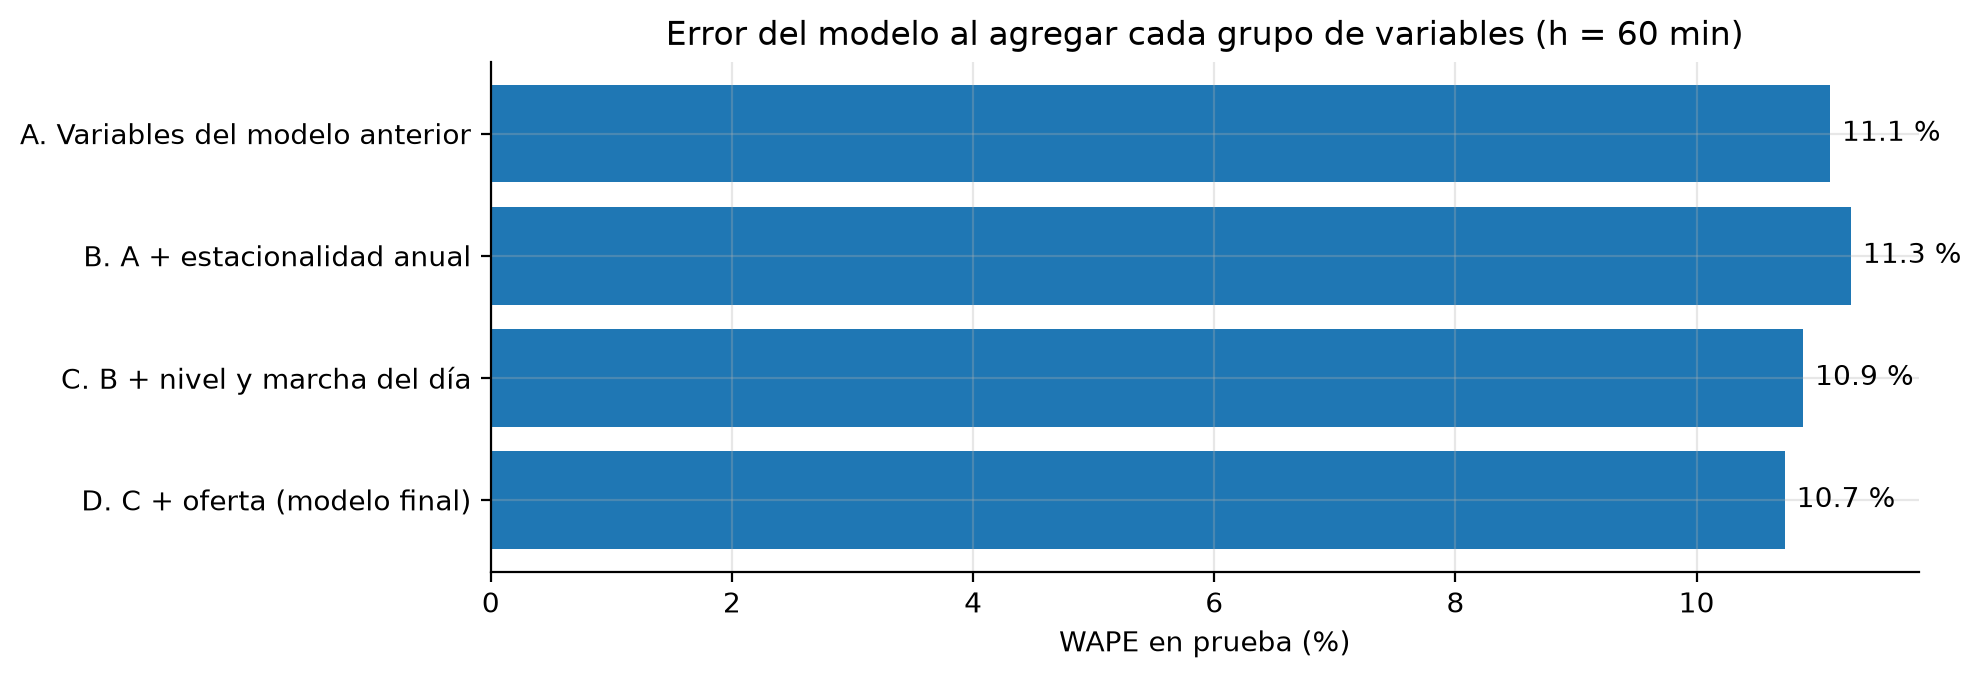
\includegraphics[width=0.85\textwidth]{fig/ablacion.png}
  \caption{Error del modelo (WAPE en prueba, $h=60$ min) al agregar cada grupo de variables.}
  \label{fig:ablacion}
\end{figure}

El resultado principal es que \textbf{la mayor mejora viene de los datos y no de las variables nuevas}: con las mismas 15 variables, pero entrenadas con los tres años de sensores limpios, el WAPE baja de cerca de 40\,\% a 11,1\,\%. Las variables adicionales aportan una mejora pequeña pero consistente, hasta 10,7\,\%. Repetido con tres semillas, el conjunto completo supera al conjunto sin estacionalidad anual en las nueve combinaciones de horizonte y semilla, por 0,06 a 0,10 puntos porcentuales, con una desviación entre semillas de 0,01 a 0,03 puntos. Cabe notar que añadir solo la estacionalidad anual (B) no mejora por sí sola el WAPE total en una sola ejecución; su ventaja aparece en la comparación del conjunto completo repetida con varias semillas.

\subsection{Importancia de las variables}

La Figura~\ref{fig:shap} muestra el impacto medio absoluto de cada variable según SHAP para $h=60$ minutos. El promedio de cuatro semanas, la hora del día y el último dato conocido explican la mayor parte de cada predicción, seguidos por la oferta de viajes (reciente y habitual), el dato del día anterior y el tipo de día. A 30 minutos, \texttt{lag\_h} es la variable más importante; a 120 minutos ya no figura entre las cinco primeras y dominan el patrón habitual (\texttt{prom\_4\_semanas}, \texttt{minuto\_dia}) y la oferta habitual (\texttt{viajes\_habituales}). Esto respalda la decisión de entrenar un modelo por horizonte. Las variables de Carnaval y Precarnaval tienen importancia casi nula únicamente porque el periodo de prueba (junio a diciembre) no contiene Carnaval.

\begin{figure}[H]
  \centering
  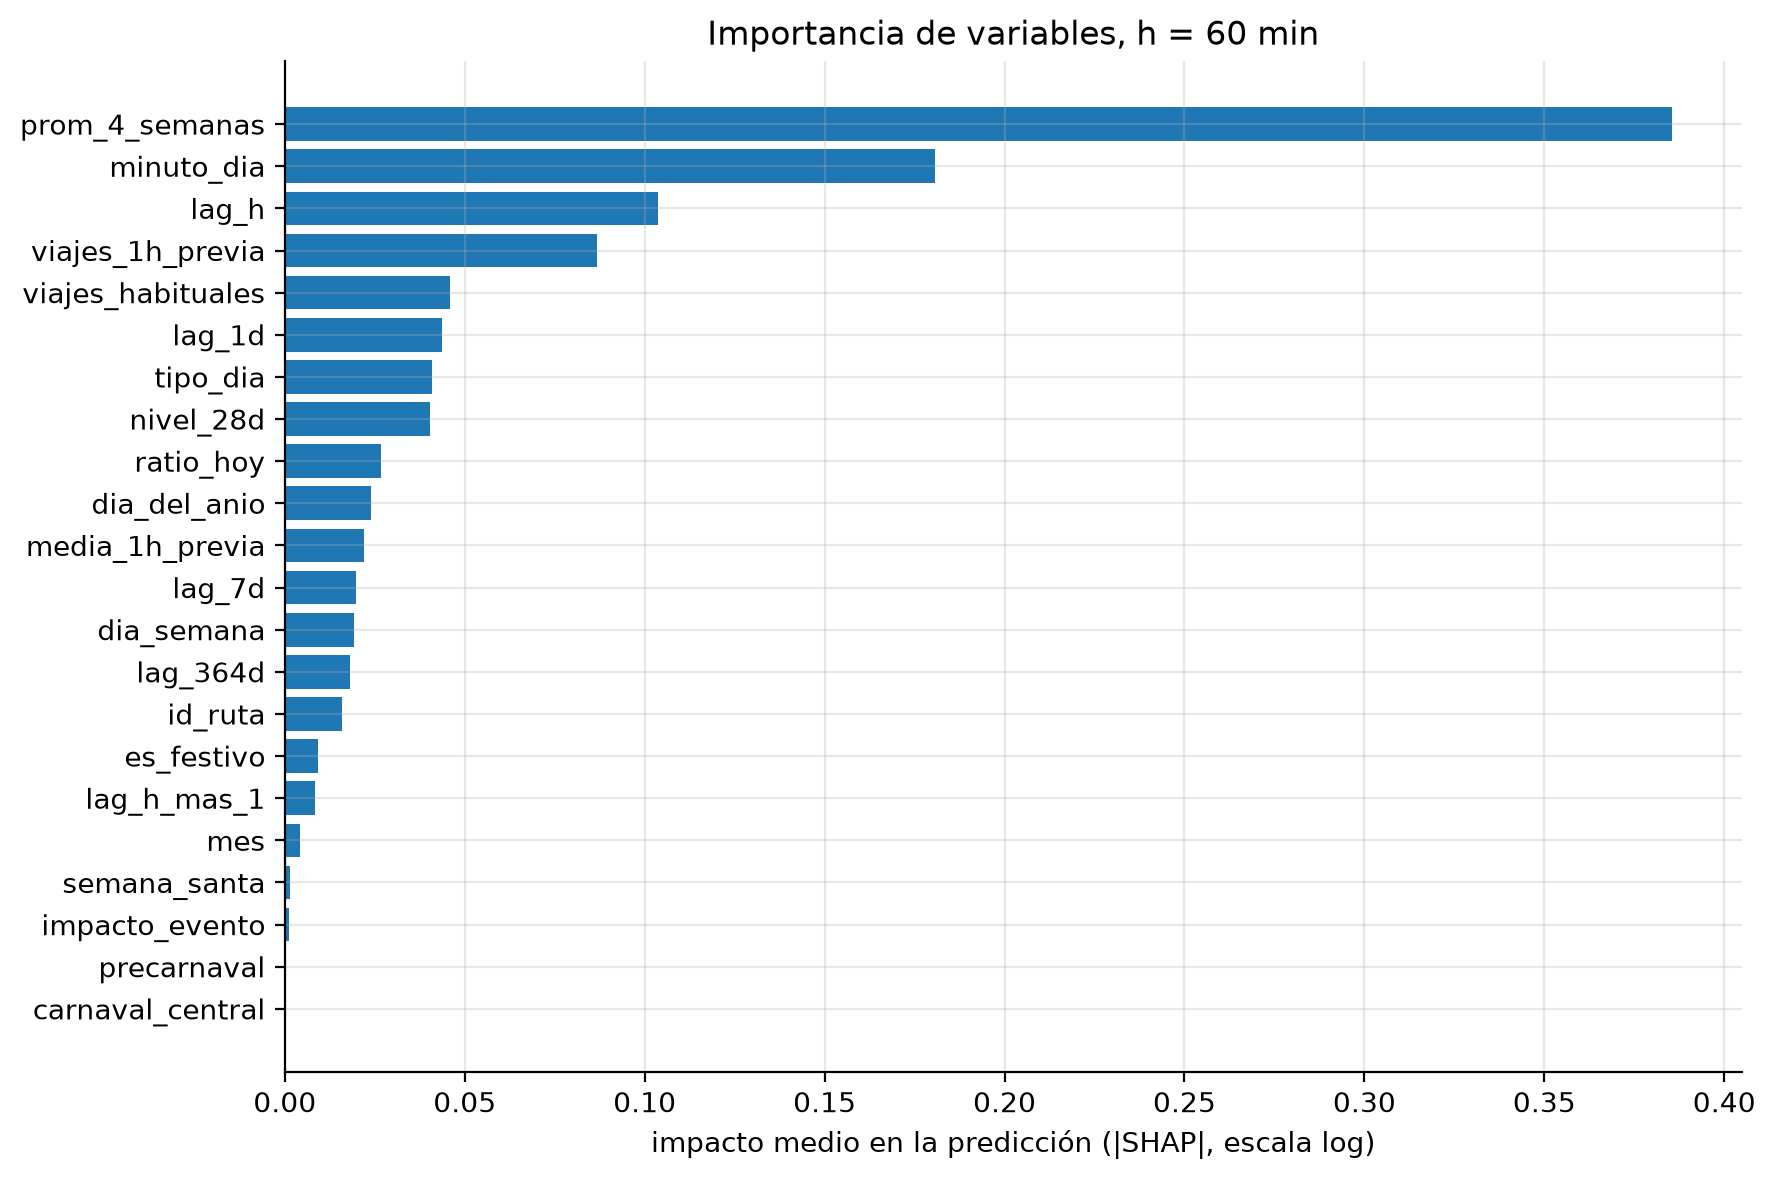
\includegraphics[width=0.75\textwidth]{fig/shap.png}
  \caption{Importancia de las variables según SHAP (impacto medio absoluto en la predicción), $h=60$ min.}
  \label{fig:shap}
\end{figure}

\subsection{Resultados por ruta y por tipo de día}

La Tabla~\ref{tab:desglose} desglosa el WAPE de prueba de los mismos modelos de la Tabla~\ref{tab:resultados}.

\begin{table}[H]
  \centering
  \caption{WAPE en prueba por ruta y por tipo de día: línea base (promedio de 4 semanas) $\rightarrow$ XGBoost. \emph{Especial} agrupa festivos, Carnaval y Semana Santa (1\,988 franjas); \emph{normal}, 43\,956 franjas.}
  \label{tab:desglose}
  \small
  \begin{tabular}{lccc}
    \toprule
     & 30 min & 60 min & 120 min \\
    \midrule
    Ruta 2 (Silencio)  & 16,2 $\rightarrow$ 10,8\,\% & 16,2 $\rightarrow$ 11,2\,\% & 16,2 $\rightarrow$ 11,5\,\% \\
    Ruta 16 (Cra. 54)  & 14,4 $\rightarrow$ 8,6\,\%  & 14,4 $\rightarrow$ 9,1\,\%  & 14,4 $\rightarrow$ 9,4\,\% \\
    Ruta 21 (Cl. 72)   & 19,5 $\rightarrow$ 14,6\,\% & 19,5 $\rightarrow$ 14,9\,\% & 19,5 $\rightarrow$ 15,3\,\% \\
    \midrule
    Días normales      & 13,7 $\rightarrow$ 10,2\,\% & 13,7 $\rightarrow$ 10,6\,\% & 13,7 $\rightarrow$ 10,9\,\% \\
    Días especiales    & 113,1 $\rightarrow$ 15,4\,\% & 113,1 $\rightarrow$ 16,5\,\% & 113,1 $\rightarrow$ 17,5\,\% \\
    \bottomrule
  \end{tabular}
\end{table}

\paragraph{Por ruta.} El modelo mejora en las tres rutas y en todos los horizontes. La Ruta 16, la de mayor volumen, es la más predecible (8,6--9,4\,\%); la Ruta 21, la de menor demanda, es la más difícil (14,6--15,3\,\%), probablemente porque con menos pasajeros por franja el ruido relativo es mayor.

\paragraph{Días especiales.} En días normales el error es de 10,2--10,9\,\%. En días especiales sube a 15,4--17,5\,\%, pero la línea base del promedio de cuatro semanas se equivoca en 113,1\,\%: promedia semanas sin festivo y proyecta una demanda de día hábil sobre un día que se comporta como domingo. Esta es la mayor ganancia relativa del modelo y proviene de las variables de calendario y de la marcha del día.

%-----------------------------------------------------------------------
\section{Despliegue}
\label{sec:despliegue}
%-----------------------------------------------------------------------

Los modelos se guardan con sus metadatos (identificador, versión de variables, lista de variables, horizonte, fecha de corte de los datos, cortes de validación y prueba, número de árboles, semilla y métricas) y se sirven mediante un servicio FastAPI. El modelo que se sirve es el reentrenado con los tres años completos, de modo que incorpora los patrones más recientes, hasta diciembre de 2025. Al arrancar, el servicio carga la copia local de los datos ya limpios con las mismas reglas del entrenamiento y calcula las variables con la misma función usada para entrenar, de modo que el modelo recibe al predecir exactamente lo que vio al aprender. El servicio rechaza modelos entrenados con una versión de variables distinta a la del código, para evitar predicciones erróneas silenciosas, y no predice si no hay datos en las 48 horas previas, lo que cubre el día sin sensor de fin de mes.

%-----------------------------------------------------------------------
\section{Discusión y limitaciones}
%-----------------------------------------------------------------------

\begin{itemize}
  \item \textbf{Alcance.} El estudio cubre tres rutas; la generalización a otras rutas no está probada.
  \item \textbf{Periodo de prueba sin Carnaval.} El desempeño en esa temporada, la de mayor alteración, no se evaluó fuera de muestra.
  \item \textbf{Hiperparámetros fijos.} No se hizo búsqueda de hiperparámetros y los modelos finales usan una sola semilla.
  \item \textbf{Sin incertidumbre.} El modelo entrega una predicción puntual, sin intervalos de confianza.
\end{itemize}

%-----------------------------------------------------------------------
\section{Conclusiones}
%-----------------------------------------------------------------------

Con tres años de lecturas de sensores correctamente limpiadas y variables sin fuga de información, un XGBoost con objetivo de Poisson predice las subidas de pasajeros por ruta y franja de 15 minutos con un WAPE de 10,3\,\% a 30 minutos, 10,7\,\% a 60 minutos y 11,1\,\% a 120 minutos, entre 30\,\% y 35\,\% mejor que el promedio de las cuatro semanas previas. La conclusión más relevante es práctica: la calidad y la cobertura temporal de los datos pesaron más que la sofisticación de las variables. El dato reciente es decisivo a 30 minutos, mientras que a 120 minutos domina el patrón habitual, lo que justifica un modelo por horizonte.

%-----------------------------------------------------------------------
\section*{Disponibilidad de datos y código}
%-----------------------------------------------------------------------

El código de extracción, limpieza, entrenamiento y servicio, junto con los cuadernos de análisis exploratorio y de ingeniería de variables, está en el repositorio del proyecto \emph{Data Challenge}. Los datos provienen de la base del operador SOBUSA.

\begin{thebibliography}{9}

\bibitem{chen2016xgboost}
T.~Chen y C.~Guestrin,
``XGBoost: A scalable tree boosting system'',
en \emph{Proc. 22nd ACM SIGKDD Int. Conf. on Knowledge Discovery and Data Mining}, 2016, pp.~785--794.

\bibitem{lundberg2017unified}
S.~M.~Lundberg y S.-I.~Lee,
``A unified approach to interpreting model predictions'',
en \emph{Advances in Neural Information Processing Systems 30}, 2017.

\bibitem{hyndman2006another}
R.~J.~Hyndman y A.~B.~Koehler,
``Another look at measures of forecast accuracy'',
\emph{International Journal of Forecasting}, vol.~22, n.º~4, pp.~679--688, 2006.

\end{thebibliography}

\end{document}
